\begin{enumerate}
	\item Exercício
	
	Calcule a área do circulo de raio igual a dois
	
	\begin{figure}[H]
		\centering
		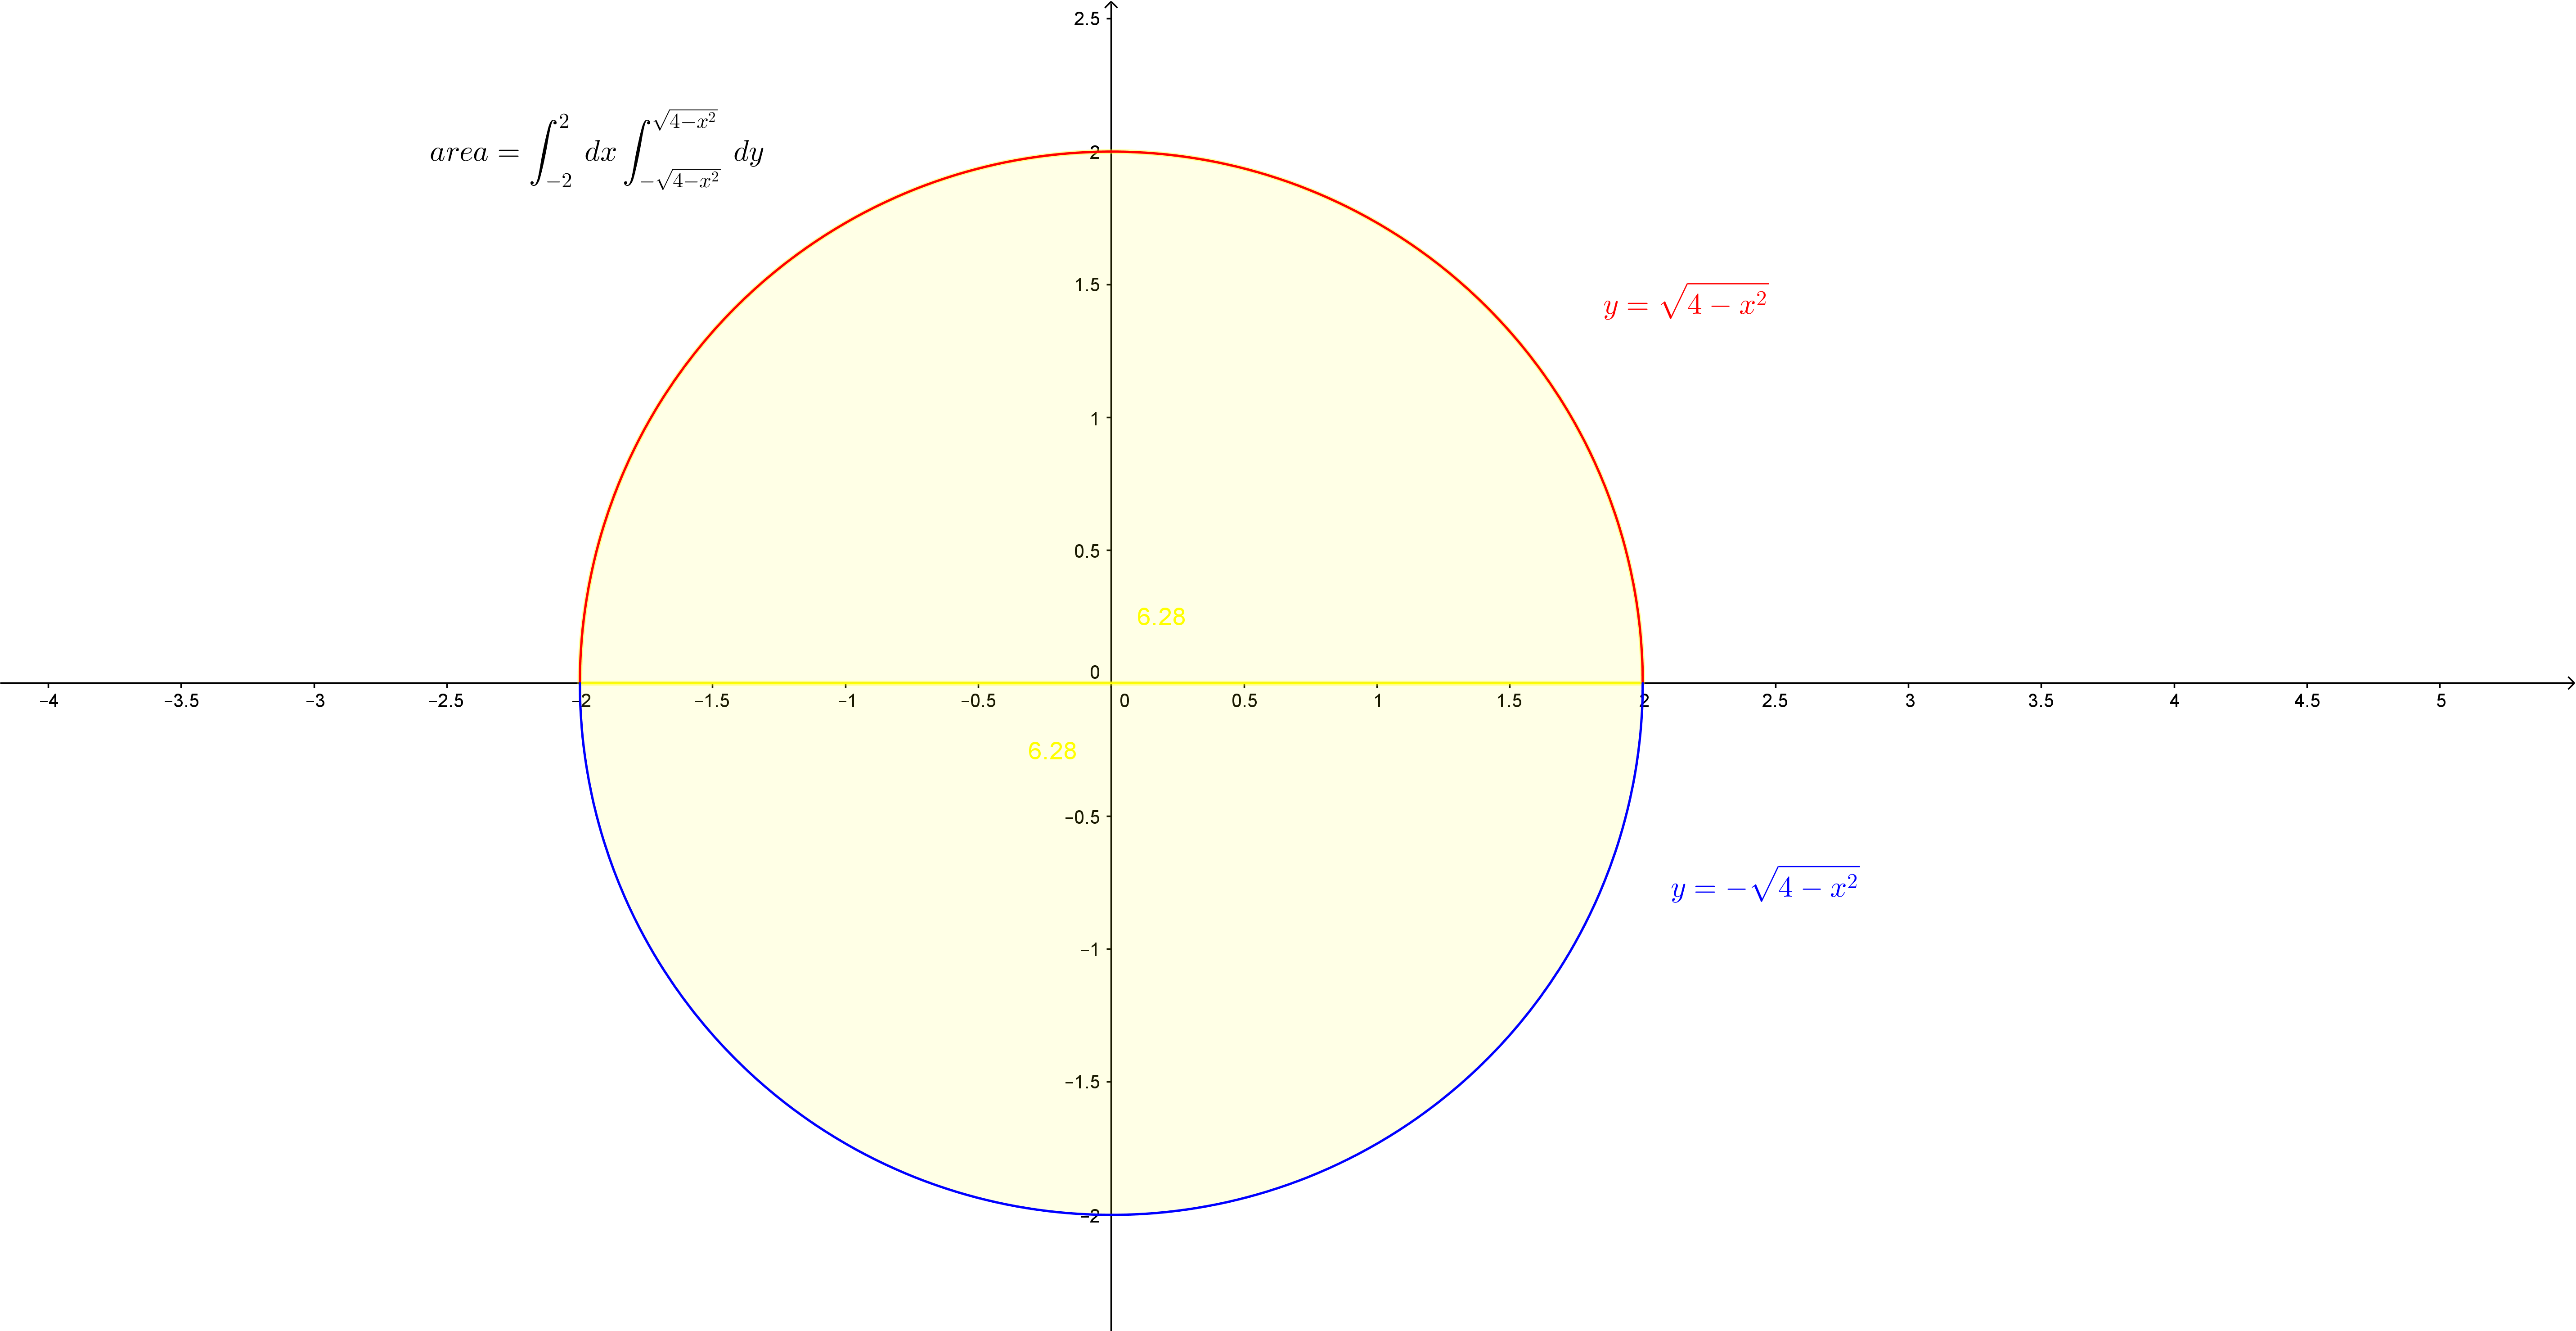
\includegraphics[width=\textwidth]{v11_a01_e01.png}
		\caption{Coordenadas polares - Aula 01 - Exercício I}
		\label{v11_a01_e01}
	\end{figure}
	
	$r = 2 \Rightarrow a = \pi r^2 = 2^2 \pi = 4\pi$\newline
	
	$x^2 + y^2 = r^2 \Rightarrow x^2 + y^2 = 2^2 \Rightarrow x^2 + y^2 = 4 \Rightarrow y = \pm\sqrt{4 - x^2}$\newline	
	$R = \left\{(x, y) \in \mathbb{R}^2 \,|\, -2 \leq x \leq 2,\, -\sqrt{4 - x^2} \leq y \leq \sqrt{4 - x^2} \right\}$\newline
	
	$a = \integral_{-2}^2 dx \integral_{-\sqrt{4 - x^2}}^{\sqrt{4 - x^2}} dy = \integral_{-2}^2 dx \left(\sqrt{4 - x^2} + \sqrt{4 - x^2}\right) = 2\integral_{-2}^2 \sqrt{4 - x^2}\, dx = 2\integral_{-2}^2 \sqrt{4 - (2\sen(\alpha))^2}\, 2\cos(\alpha)\,d\alpha = 4\integral_{-2}^2 \sqrt{4 - 4\sen^2(\alpha)}\, \cos(\alpha)\,d\alpha = 4\integral_{-2}^2 \sqrt{4 - 4\left(1 - \cos^2(\alpha)\right)}\, \cos(\alpha)\,d\alpha = 4\integral_{-2}^2 \sqrt{4 - \left(4 - 4\cos^2(\alpha)\right)}\, \cos(\alpha)\,d\alpha = 4\integral_{-2}^2 \sqrt{\overstrike{4 - 4} + 4\cos^2(\alpha)}\, \cos(\alpha)\,d\alpha = 4\integral_{-2}^2 2\cos(\alpha)\cos(\alpha)\,d\alpha = 8\integral_{-2}^2 \cos^2(\alpha)\,d\alpha = 8\integral_{-2}^2 \left(\dfrac{1 + \cos(2\alpha)}{2}\right)\,d\alpha = 8\integral_{-2}^2 \left(\dfrac{1}{2} + \dfrac{\cos(2\alpha)}{2}\right)\,d\alpha = 4\integral_{-2}^2 d\alpha + 4\integral_{-2}^2 \cos(2\alpha)\, d\alpha = 4\integral_{-2}^2 d\alpha + 4\integral_{-2}^2 \cos(u)\, \dfrac{du}{2} = 4\integral_{-2}^2 d\alpha + 2\integral_{-2}^2 \cos(u)\, du = \left[4\alpha + 2 \sen(u)\right]_{-2}^2 = \left[4\alpha + 2 \sen(2\alpha)\right]_{-2}^2 = \left[4\alpha + 4 \sen(\alpha)\cos(\alpha)\right]_{-2}^2 = \left[4\left(\alpha + \sen(\alpha)\cos(\alpha)\right)\right]_{-2}^2 = \left[4\left(\arcsen\left(\dfrac{x}{2}\right) + \dfrac{x}{2}\dfrac{\sqrt{4 - x^2}}{2}\right)\right]_{-2}^2 = \left[4\left(\arcsen\left(\dfrac{x}{2}\right) + \dfrac{x\sqrt{4 - x^2}}{4}\right)\right]_{-2}^2 = 4\left(\arcsen\left(\dfrac{2}{2}\right) + \dfrac{2\sqrt{4 - 2^2}}{4}\right) - 4\left(\arcsen\left(\dfrac{(-2)}{2}\right) + \dfrac{(-2)\sqrt{4 - (-2)^2}}{4}\right) = 4\arcsen(1) - 4\arcsen(-1) =  4(\arcsen(1) - \arcsen(-1)) = 4\left(\dfrac{\pi}{2} + \dfrac{\pi}{2}\right) = 4\left(\dfrac{\overstrike{2}\pi}{\overstrike{2}}\right) = 4\pi$\newline\newline
	$x = 2\sen(\alpha);\; dx = 2\cos(\alpha)\,d\alpha$\newline
	$u = 2\alpha;\; \dfrac{du}{2} = d\alpha$\newline\newline
	$sen(\alpha) = \dfrac{co}{h} = \dfrac{x}{2} \Rightarrow \alpha = \arcsen\left(\dfrac{x}{2}\right)$\newline
	$h^2 = co^2 + ca^2 \Rightarrow 2^2 = x^2 + ca^2 \Rightarrow ca = \sqrt{4 - x^2}$\newline
	$cos(\alpha) = \dfrac{ca}{h} = \dfrac{\sqrt{4 - x^2}}{2}$\newline
	
	$R = \left\{(r, \theta) \in \mathbb{R}^2 \,|\, 0 \leq r \leq 2,\, 0 \leq \theta \leq 2\pi \right\}$\newline
	
	$a = \integral_{-2}^2 dx \integral_{-\sqrt{4 - x^2}}^{\sqrt{4 - x^2}} dy = \integral_0^2 \integral_0^{2\pi} r\, drd\theta = \integral_0^2 r\, dr \integral_0^{2\pi} d\theta = \left[\dfrac{r^2}{2}\right]_0^2 [\theta]_0^{2\pi} = \dfrac{1}{2}\left[2^2 - 0^2\right][2\pi - 0] = \dfrac{4}{\overstrike{2}}\overstrike{2}\pi = 4\pi$\newline
	
	\item Exercício
	
	$\iintegral_R \dfrac{da}{1 + x^2 + y^2}$
	
	\begin{figure}[H]
		\centering
		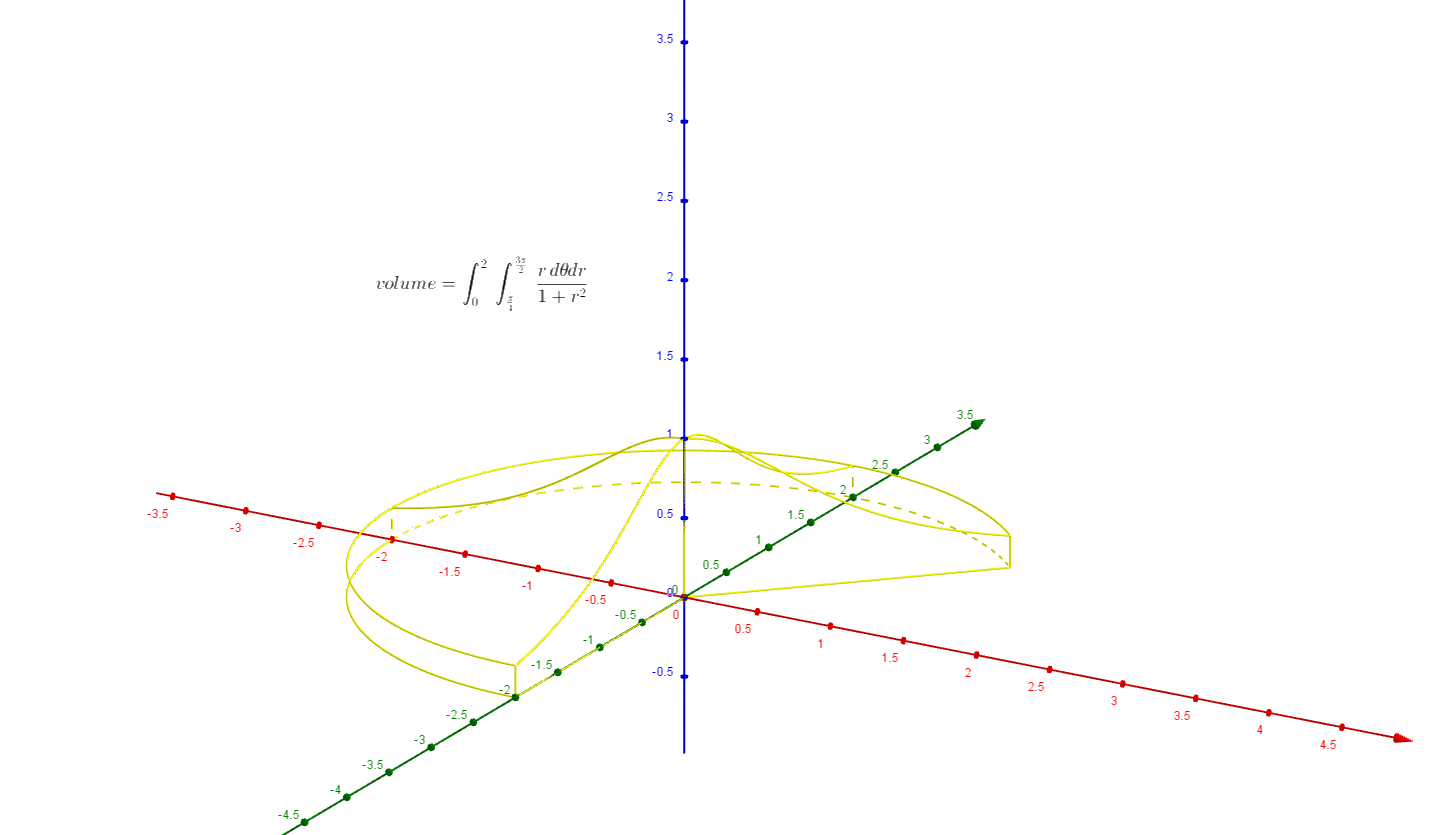
\includegraphics[width=\textwidth]{v11_a01_e02.png}
		\caption{Coordenadas polares - Aula 01 - Exercício II}
		\label{v11_a01_e02}
	\end{figure}
	
	$R = \left\{(r, \theta) \in \mathbb{R}^2 \,|\, 0 \leq r \leq 2,\, \dfrac{\pi}{4} \leq \theta \leq \dfrac{3\pi}{2} \right\}$\newline
	$v = \iintegral_R \dfrac{da}{1 + x^2 + y^2} = \integral_0^2 \integral_{\frac{\pi}{4}}^{\frac{3\pi}{2}} \dfrac{r\, drd\theta}{1 + r^2} = \integral_0^2 \dfrac{r\, dr}{1 + r^2} \integral_{\frac{\pi}{4}}^{\frac{3\pi}{2}} d\theta = \integral_0^2 \left(1 + r^2\right)^{-1} r\, dr \left[\theta\right]_{\frac{\pi}{4}}^{\frac{3\pi}{2}} = \integral_0^2 \left(1 + r^2\right)^{-1} r\, dr \left(\dfrac{3\pi}{2} - \dfrac{\pi}{4}\right) = \integral_0^2 \left(1 + r^2\right)^{-1} r\, dr\left(\dfrac{6\pi - \pi}{4}\right) = \dfrac{5\pi}{4}\integral_0^2 \left(1 + r^2\right)^{-1} r\, dr = \dfrac{5\pi}{4}\integral_0^2 u^{-1} \dfrac{du}{2} = \dfrac{5\pi}{8}\integral_0^2 u^{-1} du = \dfrac{5\pi}{8}\left[ln |u|\right]_0^2 = \dfrac{5\pi}{8}\left[ln |1 + r^2|\right]_0^2 =\\ \dfrac{5\pi}{8}\left[ln |1 + 2^2| - ln |1 + 0^2|\right] = \dfrac{5\pi}{8}\left[ln |5| - ln |1|\right] = \dfrac{5\pi ln |5|}{8}$\newline\newline
	$u = 1 + r^2 \Rightarrow \dfrac{du}{2} = r\,dr$\newline
	$\e^x = 1 = \e^0 \Rightarrow x = 0$\newline	
\end{enumerate}
